%% outhesis_template.tex
%% version 1.1
%% Chris McRaven <mcraven@physics.ou.edu>
%% With updates from Leah Morabito <morabito@nhn.ou.edu>
%%
%% 'outhesis.cls' is a class file for a master or phd thesis that
%% conforms to the requirements of the graduate college at the
%% University of Oklahoma. This file is a hacked version of 'book.cls,'
%% that includes all of the formatting requirements set forth in
%% the document 'DissertationInstPacket.pdf' available at
%% http://gradweb.ou.edu/Current/Forms/doctoral/DissertationPagination.pdf
%%
%% This class file relies on a few packages to work.  You must have the
%% following packages installed:
%%  amsfonts, amsmath, amssymb, tikz, lineno, microtype, hyperref
%%
%% Most of these packages are included in distributions of latex.  If you
%% get alot of errors when compiling, check that these packages are
%% installed.
%%
%% By default, the class file will conform to the requirements, but three
%% options are provided for assistance in proofing the document.
%%
%% linenumbers -- turns on linenumbers in the left margin
%% summarypage -- places a page at the beginning of the document listing 
%%                the number of tables, figures, and bibliography items.
%% hyperlinks -- hyperlinks the citations and references for easier
%%                navigation in the document in a reader which supports
%%                hyperlinks.
%%
%% NOTE FOR MASTERS STUDENTS: Open the outhesis.cls file, find the word 
%% "DISSERTATION" and replace with "THESIS" and then save.
%%
% \documentclass[linenumbers,summarypage,hyperlinks]{outhesis}
\documentclass{outhesis}

% For a bibliography style, you must have the appropriate .bst file
% \bibliographystyle{apj}
\bibliographystyle{prsty}

% Provide the correct margins
\usepackage[top=1in, bottom=1in, left=1.6in, right=1.2in]{geometry}
% If you want a double-sided copy for yourself, uncomment the next line
% \usepackage[twoside,top=1in, bottom=1in, left=1.6in, right=1.2in]{geometry}


\begin{document}

%% Place Dissertation information here
%% Follow the convention for the use of capital letters 
%% or else the font will not be formatted properly
\author{Othmane Rifki}
\university{UNIVERSITY OF OKLAHOMA}
\college{GRADUATE COLLEGE}
\department{DEPARTMENT OF PHYSICS AND ASTRONOMY}

\title{In Search for New States of Matter using the ATLAS Detector at the Large Hadron Collider at CERN}

\address{Norman, Oklahoma}
\yr{2010}
\dgname{DOCTOR OF PHILOSOPHY}
%% List your committee members here
\committee{{Dr. Brad Abbott, Chair}, Mrs. Eleanor Roosevelt, {Mr. Junior Senior, Jr.}, Dr. Dre}

%% Put your dedication here. This is completely optional. Delete it if you don't need it.
\begin{dedication}
  To my loving cats, oh, how I do love you so.
\end{dedication}

%% Put your acknowledgements here. This is completely optional. Delete it if you don't need it.
\begin{acknowledgements}
  I would like to acknowledge the National Basketweaving Foundation and the University of Oklahoma for funding this work. Also, my friend Doug.
\end{acknowledgements}

%% Put your abstract here.

\begin{abstract}
A new, Earth-shattering weave design is presented.
Called the ``Wicked--Googly Weave,'' this novel weave is weaverific and will revolutionize baskets and their construction while immersed in water.
\end{abstract}


\frontmatter

\maketitle

\mainmatter

\chapter{Introduction}

\section{Implications}

Basket-weaving is a fine art begun over five million years ago by the eskimos.
For many decades, they toiled to perfect their magical baskets.
It is said that they could weave a basket around a killer whale and not get wet.
The Great Flood almost wiped all record of their activities if not for Squanto~\cite{Doug}.
Recently, more esoteric weaves have elucidated the matter-antimatter asymmetry in the universe~\cite{Lee+1957}.

\section{Compatibility}

You have to fight to get to the top of the basket-weaving world (See Figure~\ref{fig:training}.)
The formed basket must be compatible with its place of placement.
Refer to Table~\ref{tab:baskets} for a brief compatibility list.

\begin{figure}
  \centering
  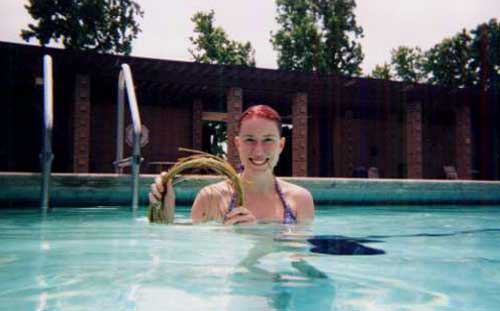
\includegraphics[scale=0.5]{figures/ubw}
  \caption{An extreme training session.}
  \label{fig:training}
\end{figure}


\begin{table}
  \caption{Tables and their basket holding capability.}
  \label{tab:baskets}
  \centering
  \begin{tabular}{l}
    \begin{tabular*}{0.6\textwidth}{l @{\extracolsep{\fill}} l} \hline \hline
      Table shape   & BHC$^{\dagger}$ \\ \hline
      Rect-angular  & YES \\
      Square        & YES \\
      Round         & YES$^{\ddagger}$ \\
      Water         & NO \\ \hline
    \end{tabular*} \\
    $^{\dagger}$ BHC -- Basket Holding Capability \\
    $^{\ddagger}$ Tables with knights should be avoided. \\
  \end{tabular}
\end{table}

%% You can put any part of the text in separate file with 
%% the \input{} command. This keeps the master document simpler.


\chapter{The wicked--googly weave}

\section{Introduction}

The wicked--googly weave (WiGoo) is technologically superior to all previous weaves~\cite{Science}.
Although the WiGoo provides +4 shield bonus and protects against incorporeal touch attacks, it is not very effective against ninturpoos (See Figure~\ref{fig:ninturpoos}.)

\begin{figure}
  \centering
  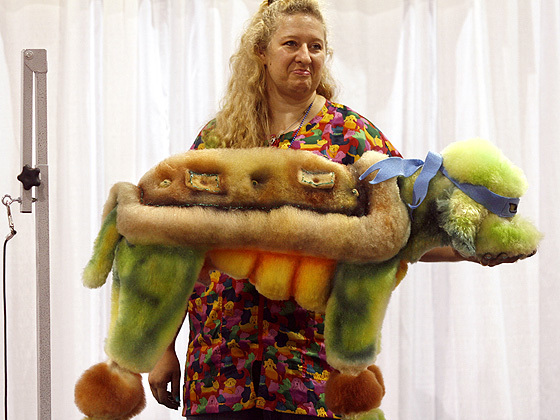
\includegraphics[scale=0.5]{figures/ntp}
  \caption{Though rare, ninja turtle poodles, or ninturpoos, are particularly devastating to baskets.}
  \label{fig:ninturpoos}
\end{figure}


\section{This stuff is for real}

The WiGoo method can seriously whip out some serious basket.
A quite serious basket is shown in Figure~\ref{fig:serious}.

\begin{figure}
  \centering
  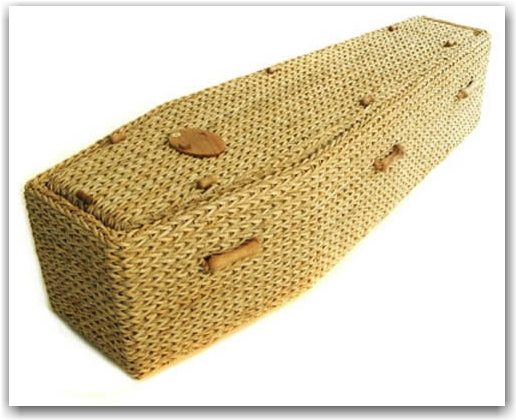
\includegraphics[scale=0.5]{figures/sbskt}
  \caption{This basket was woven woefully in under 26.2 seconds.}
  \label{fig:serious}
\end{figure}


%% You need a file named `outhesis_references.bib' to use BibTex here
\bibliography{outhesis_references}

% \appendix
% \input{appendices/appenda}
% \input{appendices/appendb}

% \backmatter


\end{document}


